\documentclass{article}
\usepackage{tikz}
\usetikzlibrary{shapes.geometric, arrows}

% Define block styles
\tikzset{
    block/.style = {rectangle, draw, fill=blue!20, 
                    text width=5em, text centered, rounded corners, minimum height=4em},
    line/.style = {draw, -latex'},
    cloud/.style = {draw, ellipse,fill=red!20, node distance=3cm,
                    minimum height=2em}
}

\begin{document}

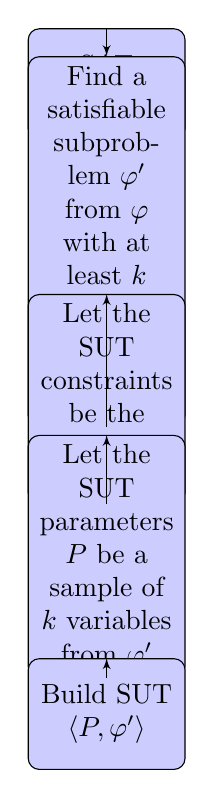
\begin{tikzpicture}[node distance = 2cm, auto]
    % Place nodes
    \node [block] (init) {SAT instance $\varphi$};
    \node [block, below of=init] (subproblem) {Find a satisfiable subproblem $\varphi'$ from $\varphi$ with at least $k$ variables and of at least some hardness};
    \node [block, below of=subproblem] (constraints) {Let the SUT constraints be the clauses in $\varphi'$};
    \node [block, below of=constraints] (parameters) {Let the SUT parameters $P$ be a sample of $k$ variables from $\varphi'$};
    \node [block, below of=parameters] (sut) {Build SUT $\langle P, \varphi' \rangle$};

    % Draw edges
    \path [line] (init) -- (subproblem);
    \path [line] (subproblem) -- (constraints);
    \path [line] (constraints) -- (parameters);
    \path [line] (parameters) -- (sut);
\end{tikzpicture}

\end{document}